I collected two different types of data for 143 dispute cases 
requested to the WTO DSB.
One is textual description of trade policy 
that led to the dispute and the other one is 
set of articles of the WTO agreement that are
cited for each dispute. 
I will explain the format and the content of 
each type of data with an example. 
Technical details about automated way 
of collecting and cleansing the data is 
explained in \ref{sec:appendix}

\begin{figure}
    \centering
    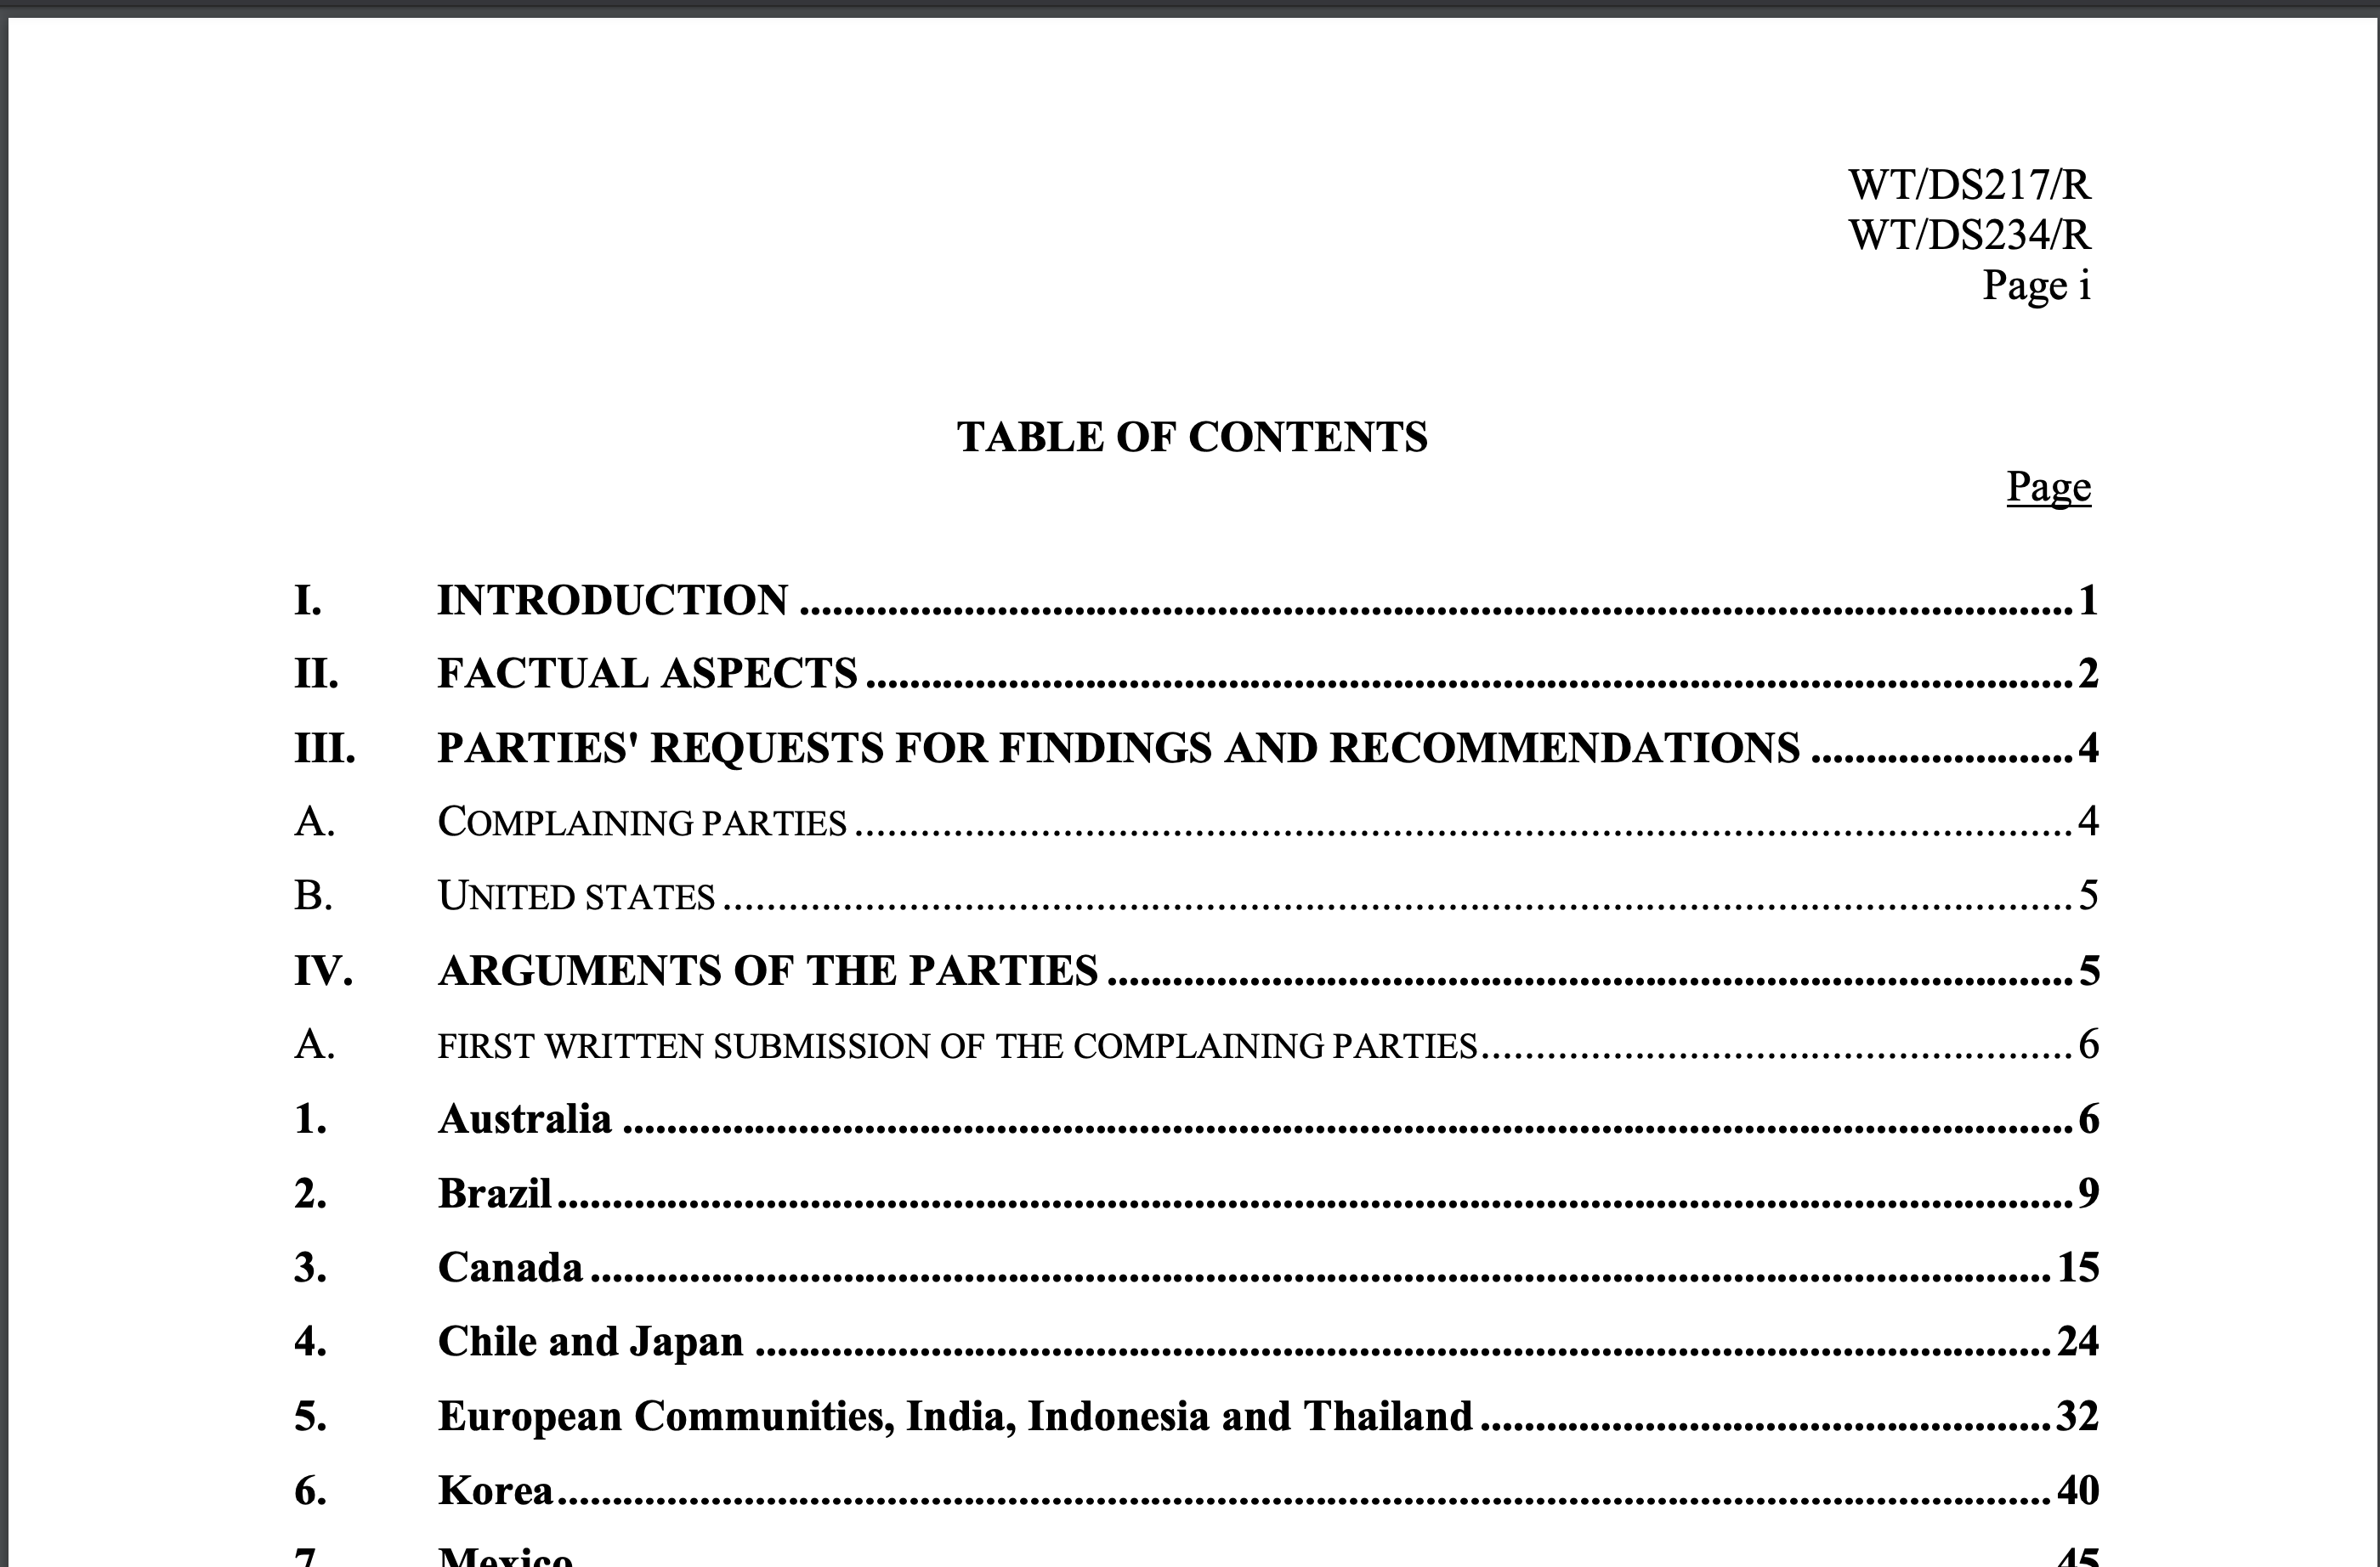
\includegraphics[scale=0.2]{Data/pngs/panel_report_toc.png}
    \caption{{\bf Table of Contents of the Panel Report: }It shows {\bf FACTUAL ASPECTS} and we have linked cases because of the judicial economy }
\end{figure}



% This section explains how I collected 
% which data to train the neural network. 
% Basically, 





% I collected two different 
% types of data, one is textual description of trade policy 
% that led to the dispute and the other one is 
% set of articles of the WTO agreement that are
% cited for the dispute.s



% \begin{displayquote}
%     ``Korea' s domestic support for beef in 1997 and 1998 exceeded the de minimis level contrary to Article 6 of the Agreement on Agriculture.''
%   \end{displayquote}
  
%   \begin{itemize}
%     \item exemplify as detail as possible to inform readers about how data looks like.
%     \item Privide a running example that shows how WTO works with data. 
%     \item (Borrow from the previous paper)
    
%   \end{itemize}
  